\section{Evaluation}
\label{sec:evaluation}

\subsection{Experimental Setup}
\label{sec:evaluation.setup}

We implemented our dataflow-guided monitoring architecture by
modifying the ARM version of the gem5 simulator \cite{gem5} to support parallel
run-time monitoring. We model the main and monitoring cores as running at 2.5
GHz with 4-way set-associative private L1 I/D caches and a shared 8-way 2 MB L2
cache. This setup is similar to the Snapdragon 801 processor commonly found in
mobile systems. The dataflow engine uses a 1 kB cache for flags.

In order to explore the generality of the architecture for
different monitors, we implemented three different monitors: uninitialized
memory check (UMC), array bounds check (BC), and dynamic information flow
tracking (DIFT).  Uninitialized memory check seeks to detect loading from
memory locations that are not initialized first.  Array bounds check, as
mentioned in Section~\ref{sec:monitoring}, is a monitoring scheme that aims to
detect buffer overflows where memory accesses go beyond the boundaries of an
array. We modify the implementation of {\tt malloc} to set base and bound
metadata information. Dynamic information flow tracking is a security
monitoring scheme
which detects when information from untrusted sources is used to affect the
program control flow (i.e., indirect control instructions). For the benchmarks we consider, we mark data read from
files as untrusted. We implemented a multi-bit DIFT scheme which marks
untrusted data with a 32-bit metadata identifier so
that if an error is detected, it is possible to have information about where
the data originated from. 

We tested our system using all C benchmarks from SPECint
CPU2006 \cite{spec2006}. Since our implementation of BC depends on the
modification of {\tt malloc} to set array bounds information, we focus on the C
SPECint benchmarks. Although we do not
show results for the C++ benchmarks, we note that the results for UMC and DIFT
for these benchmarks are similar to the other results shown. For each
benchmark, we simulated for 1 billion instructions. An initial slack of 1
million cycles, which is less than 1\% of
the total execution time, is given for a 10\% target overhead. This initial
slack is scaled proportionally for other overhead targets.

\subsection{Baseline Monitoring Overheads}
% Full monitoring overheads
\begin{figure}
  \begin{center}
    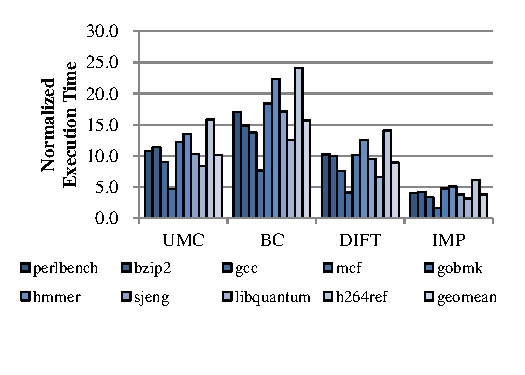
\includegraphics[width=\columnwidth]{figs/data_full_mon.pdf}
    \vspace{-0.2in}
    \caption{Full monitoring overheads for UMC, BC, and DIFT.}
    \label{fig:evaluation.full_mon}
    \vspace{-0.1in}
  \end{center}
\end{figure} Figure~\ref{fig:evaluation.full_mon} shows the execution times of
performing full monitoring normalized to the execution times of the benchmarks
without monitoring. In these results, no filtering or partial monitoring is
done. UMC shows normalized execution times from 4x to 11x with an average
of 7x. BC shows normalized execution times of 9-28x with an average of
18x while DIFT shows normalized execution times of 6x-17x with an average of
11x. One of the reasons for these high overheads is that our implementations of
these monitors dynamically allocate memory for new metadata. This can be an
expensive, many-cycle operation. Statically allocating memory for metadata
will reduce the execution time but requires a large upfront memory footprint
which caused issues with our simulator.

\subsection{Filtering of Monitoring Events}

% Full monitoring overheads
\begin{figure}
  \begin{center}
    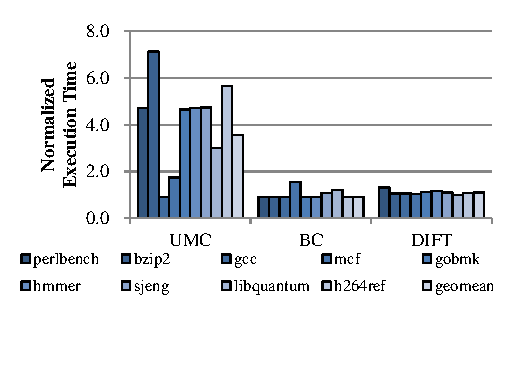
\includegraphics[width=\columnwidth]{figs/data_filtering.pdf}
    \vspace{-0.2in}
    \caption{Monitoring overheads with filtering null metadata for UMC, BC, and DIFT.}
    \label{fig:evaluation.filtering}
    \vspace{-0.1in}
  \end{center}
\end{figure}

Figure~\ref{fig:evaluation.filtering} shows the
normalized execution times with filtering enabled. We see significant
reductions in overhead for all three monitoring schemes. UMC sees normalized
execution times of 2-6x with an average of 4x with null metadata filtering.
This is an average reduction in overheads of 52\%. For BC, normalized execution
times drop from 18x down to 4x on average (an 82\% reduction). The range of normalized execution
times for filtered BC is 1.1-17x. This is not surprising since in the baseline
implementation all loads and stores needed to be monitored. However, with
filtering, only loads and stores corresponding to arrays need to be forwarded.
Finally, DIFT sees the largest reduction in overheads with only 13\% overheads
on average after filtering, a 90\% reduction in monitoring overheads, with a
maximum overhead of 42\% after filtering. This is due, in part, to the fact
that
for our implementation of DIFT on SPEC
benchmarks, we only mark data read from files as tainted. For most of these
benchmarks, this propagates to relatively few instructions. Instead, if we
targeted network or streaming applications, which have larger amounts of
untrusted input data, we would expect to see less filtering.

\subsection{Coverage with Adjustable Partial Monitoring}

% BC sweep
\begin{figure*}
  \begin{center}
    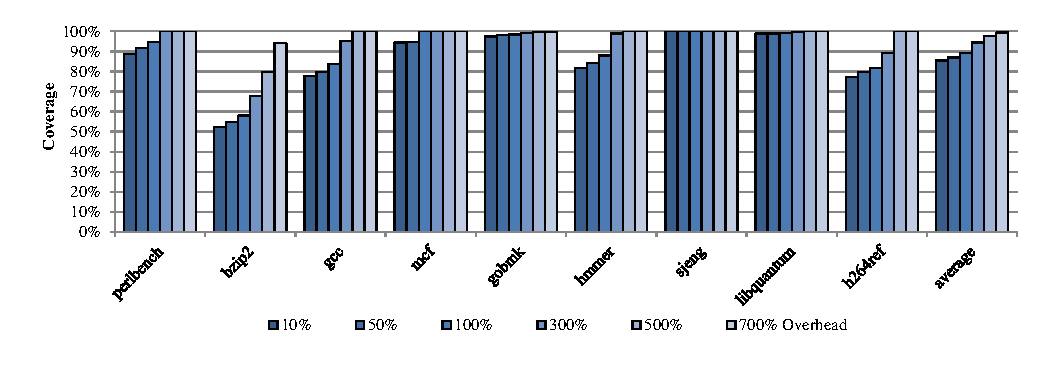
\includegraphics[width=\linewidth]{figs/data_bc_sweep.pdf}
    \vspace{-0.4in}
    \caption{Coverage versus varying overhead budget for array bounds check.}
    \label{fig:evaluation.bc_sweep}
    \vspace{-0.2in}
  \end{center}
\end{figure*}

% UMC sweep
\begin{figure*}
  \begin{center}
    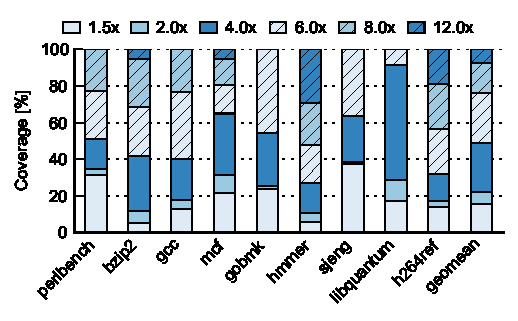
\includegraphics[width=\linewidth]{figs/data_umc_sweep.pdf}
    \vspace{-0.4in}
    \caption{Coverage versus varying overhead budget for uninitialized memory check.}
    \label{fig:evaluation.umc_sweep}
    \vspace{-0.1in}
  \end{center}
\end{figure*}

Although the overheads of DIFT are quite low after filtering, BC and UMC still
show significant overheads. In this section, we evaluate the effectiveness of
using partial monitoring (in addition to filtering) to trade-off coverage for further reduced overheads.
Figure~\ref{fig:evaluation.bc_sweep} shows the monitoring coverage achieved by
array bounds check as we vary the overhead budget. 
We define \emph{monitoring coverage} as the 
percentage of checks that are performed 
(indirect jumps in DIFT, loads in UMC, and memory accesses in BC). 
The metric is chosen to understand
how likely an error/attack instance is to be detected on an individual system. 
While we could not evaluate real errors/attacks due to difficulty in setting up
a large number of bugs and exploits, we believe that the percentage of checks
provides a good estimate of detection probability when errors/attacks are 
uniformly distributed across checks.
Note that this metric is different from the
percentage of monitoring events that are not dropped, which includes
non-check instructions.

We see that by varying the overhead budget, the coverage achieved also varies.
With only a 10\% overhead budget, array bounds check still
achieves 82\% monitoring coverage on average. The high coverage
achieved with such low overheads is due to two main effects.  The first is that
monitoring can be done in parallel, providing monitoring coverage without
introducing overheads. The second effect is that, although we aggressively
filter out monitoring events, there may still exist a large number of
monitoring events that do not lead to security or reliability checks. As a
result, dropping these events can reduce overheads without a large impact on
monitoring coverage.

Figure~\ref{fig:evaluation.umc_sweep} shows the analogous graph for UMC. Again
we see that varying overhead budgets enables partial monitoring. We see that
with a 10\% overhead budget, UMC achieves 32\% monitoring coverage on average.
By increasing this overhead budget to 50\%, UMC achieves 51\% coverage. Even
higher coverage can be achieved by allowing higher overheads.

\subsection{Comparing Dropping Policies}

% UMC exec time
\begin{figure}
  \begin{center}
    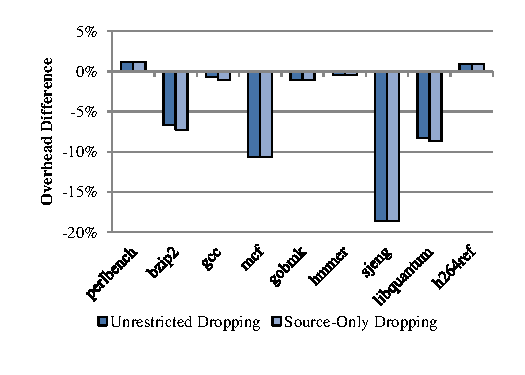
\includegraphics[width=\columnwidth]{figs/data_umc_exec_time.pdf}
    \vspace{-0.2in}
    \caption{Error in meeting overhead budget for uninitialized memory check for different dropping policies.}
    \label{fig:evaluation.umc_exec_time}
    \vspace{-0.2in}
  \end{center}
\end{figure}


% UMC coverage across policies
\begin{figure}
  \begin{center}
    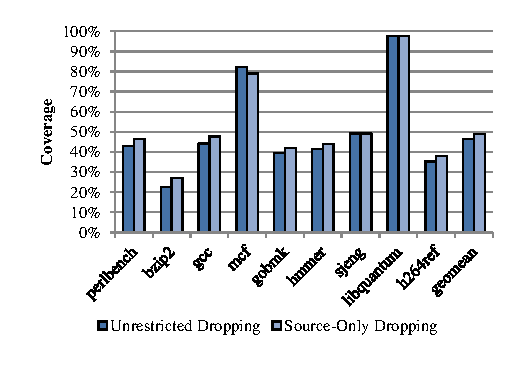
\includegraphics[width=\columnwidth]{figs/data_umc_coverage.pdf}
    \vspace{-0.2in}
    \caption{Coverage for uninitialized memory check for different dropping policies.}
    \label{fig:evaluation.umc_coverage}
    \vspace{-0.1in}
  \end{center}
\end{figure}
In this section we evaluate the trade-offs between unrestricted dropping and source-only dropping.
Figure~\ref{fig:evaluation.umc_exec_time} shows the difference between the
overhead budget and the run-time monitoring overheads for UMC. A positive value
means that the overhead target was overshot while a negative value indicates
that the overhead budget was met. We see similar results for unrestricted
dropping and source-only dropping due to the fact that UMC consists of a large
number of independent monitoring flows.
Figure~\ref{fig:evaluation.umc_coverage} shows the coverage of UMC for
unrestricted dropping and source-only dropping. We see that source-dropping
consistently achieves higher coverage than unrestricted dropping. This is due
to the fact that some of the overheads of monitoring for unrestricted dropping
are being spent on wasted work as discussed in Section~\ref{sec:policies.events}.

% BC exec time
\begin{figure}
  \begin{center}
    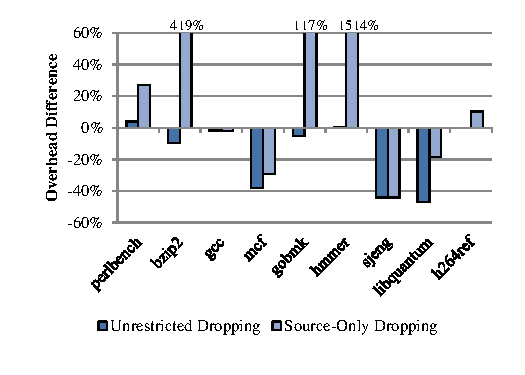
\includegraphics[width=\columnwidth]{figs/data_bc_exec_time.pdf}
    \vspace{-0.2in}
    \caption{Error in meeting overhead budget for array bounds check for different dropping policies.}
    \label{fig:evaluation.bc_exec_time}
    \vspace{-0.2in}
  \end{center}
\end{figure}

% BC coverage across policies
\begin{figure}
  \begin{center}
    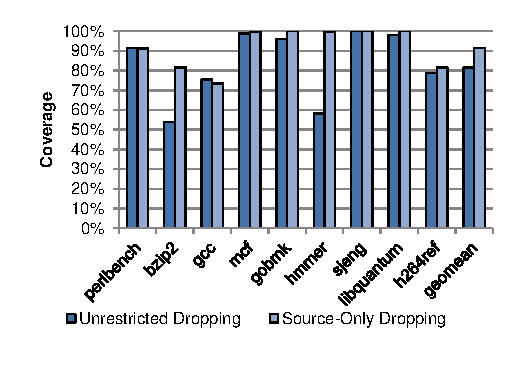
\includegraphics[width=\columnwidth]{figs/data_bc_coverage.pdf}
    \vspace{-0.2in}
    \caption{Coverage for array bounds check for different dropping policies.}
    \label{fig:evaluation.bc_coverage}
    \vspace{-0.2in}
  \end{center}
\end{figure}

Next, we evaluate these trade-offs between source-only dropping and unrestricted dropping for BC.
Figure~\ref{fig:evaluation.bc_exec_time} shows the overhead differences for BC
and Figure~\ref{fig:evaluation.bc_coverage} shows the coverage for BC.
From Figure~\ref{fig:evaluation.bc_exec_time}, we see that for several
benchmarks, source-only drop fails to meet the specified overhead target.
The overshoot of the overhead target is quite high with an overhead difference
of 420\% for {\tt bzip2}, 120\% for {\tt gcc}, and 1500\% for {\tt hmmer}.
Since only array allocations are considered source events for BC, it is
difficult for source-only dropping to match overhead targets. Although
Figure~\ref{fig:evaluation.bc_coverage} again shows higher coverage for
source-only dropping, this is in part due to the fact that is running with
higher overheads.

\subsection{Multiple-Run Coverage}

% Multi-run coverage with unrestricted dropping
\begin{figure}
  \begin{center}
    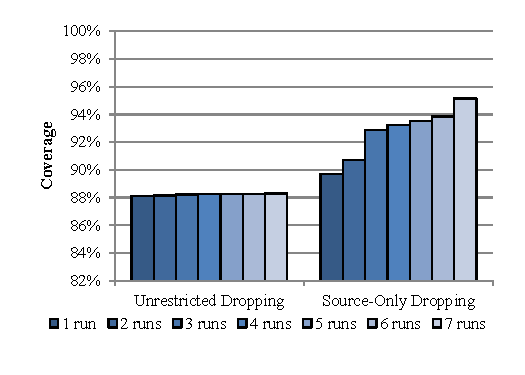
\includegraphics[width=\columnwidth]{figs/data_multirun_coverage.pdf}
    \vspace{-0.2in}
    \caption{Coverage over multiple runs for BC at 10\% overhead with an unrestricted dropping policy.}
    \label{fig:evaluation.multirun}
    \vspace{-0.1in}
  \end{center}
\end{figure}

One possible application of partial monitoring with low overheads is to enable
cooperative debugging. The idea with cooperative debugging is to use partial
monitoring with very low overheads across a large number of users or runs. By
varying the pattern of partial monitoring done on each run, the goal is to
achieve high coverage across multiple runs. Varying the monitoring that is
done for different runs can be achieved by introducing some randomness into the
dropping decision. Figure~\ref{fig:evaluation.multirun} shows the total
coverage achieved over multiple runs for array bounds check running with a 10\%
overhead budget and an unrestricted dropping policy. Each run was simulated for
100 million instructions. For these simulations, events were
dropped probabilistically with the probability scaled proportionally to slack.
That is, when slack is high, the probability of dropping is low and the
probability increases as we run out of slack. We see that the coverage achieved
quickly asymptotes for an unrestricted dropping policy. This is due to the fact
that since there are multiple dependent monitoring operations that must be done
in order for a final check to be successful, a small amount of randomness at
each event quickly compounds to reduce the probability of certain checks to
near zero. Instead, source-only dropping is much better suited for achieving high
coverage over multiple runs.

\subsection{Area and Power Overheads}

% Area and Power Overheads
\begin{table}[tb]
  \begin{center}
    \vspace{-0.0in}
    \begin{footnotesize}
    
% Full monitoring at zero slack

\begin{tabular}{|c|c|c|}
\hline

{\bf Monitor} & {\bf Peak Power [mW]} & {\bf Runtime Power [mW]} \\ \hline\hline

UMC  & 4.7 (4.9\%) &  3.1 (8.2\%) \\ \hline
BC   & 6.9 (7.1\%) &  4.1 (10.7\%) \\ \hline
DIFT & 7.2 (7.4\%) &  4.3 (11.1\%) \\ \hline

\end{tabular}

    \end{footnotesize}
    \caption{Average power overhead for dropping hardware at a 50\% overhead
    budget. Percentages in parentheses are normalized to the main core
    power.}
    \vspace{-0.2in}
    \label{tab:evaluation.area_power}
  \end{center}
\end{table}

Adding the dataflow engine in order to enable filtering and partial monitoring adds
overheads in terms of area and power. We use McPat \cite{mcpat-micro09} to get
a first-order estimate of these area and power overheads in a 40 nm technology
node. McPat estimates the main core area as 2.71 mm$^2$ and the peak power usage as
965 mW averaged across all benchmarks. The average runtime power usage was 385 
mW. These area and power numbers consist of the core and
L1 cache, but do not include L2 cache, memory controller, and other
peripherals. The power numbers include dynamic as well as static (leakage)
power. For the dataflow engine, we modeled the ALUs used for address
calculation, the dataflow flag register file and cache, the configuration
tables, and the filter decision table. These were modeled using the
corresponding memory and ALU objects in McPat. We
note that this is only a rough area and power estimate since components such as the
wires connecting these modules have not been modeled. However, this gives a
sense of the order-of-magnitude overheads involved with implementing our
approach.

Our results show that an additional 0.197 mm$^2$ of silicon area is needed, an
increase of 7\% of the main core area. Table~\ref{tab:evaluation.area_power}
shows the peak and runtime power overheads averaged across all benchmarks with
a 50\% monitoring overhead target. The peak power is 5-7 mW, which is
less than 1\% of the main core's peak power usage. Similarly, the average runtime power is 3-4 
mW, corresponding to about 1\% of the main core's runtime power.

